\chapter{Разработка}

\section{Алгоритм}
В данном подразделе рассматривается алгоритм позиционирования, начиная с того момента, когда данные об уровнях сигнала уже привязаны к точкам на маршруте, а после позиционирования не требуется осуществлять обратное преобразование. Вопрос прямого и обратного преобразования рассмотрен в подпункте \ref{subsubsec:transroute}.

\subsection{Исходные данные}
Исходными данными алгоритма являются, с одной стороны, хранящиеся в базе данных тройки $<CID, RSSI, Dist>$ (CID --- уникальный идентификатор базовой станции, RSSI --- уровень принятого сигнала от неё в точке с координатой Dist), которые были измерены ранее, и значение Dist для которых посчитано на основе данных спутниковой навигации, а с другой --- пары $<CID, RSSI>$ измеренные устройством, координаты которого требуется найти.

\begin{figure}[h]
	\center{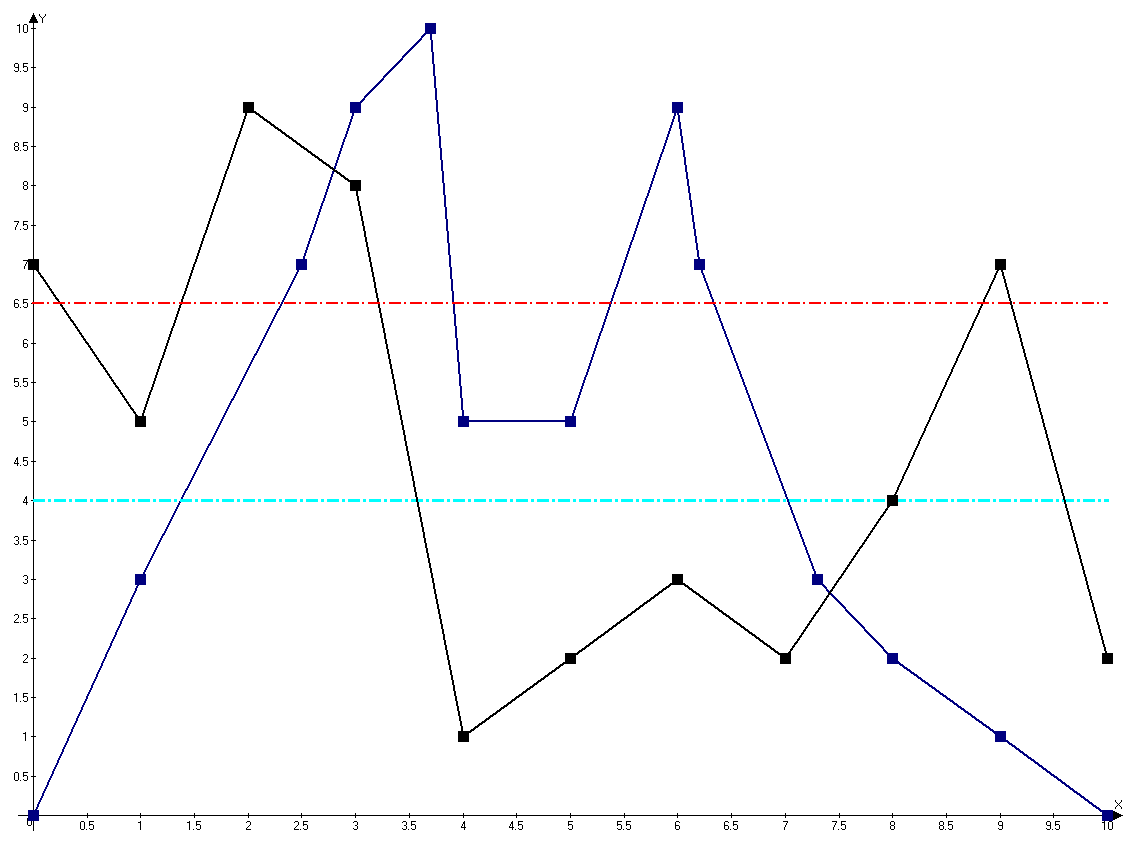
\includegraphics[width=1\linewidth]{MadMax-input.png}}
	\caption{Эскиз возможных входных данных для алгоритма позиционирования. Вертикальная ось --- уровень сигнала, горизонтальная --- координата. Штрихпунктирными линиями обозначены уровни фактически принятых сигналов от двух базовых станций (поскольку их координаты неизвестны, изображены на всём протяжении маршрута). Точки, соединённые сплошными отрезками --- хранящиеся в базе данных замеры RSSI этих станций с известными координатами.}
	\label{fig:madmax-input}
\end{figure}

Эскиз возможного вида таких данных показан на рис. \ref{fig:madmax-input}. Хранящиеся в базе данных замеры соединены прямыми линиями только для того, чтобы не путать замеры сигналов от разных станций на рисунке, реально хранятся только точки. Из базы данных осуществляется выборка тех замеров, CID которых соответствует CID фактически принятых сигналов.

\subsection{Интерполяция}
Для того, чтобы перейти от дискретной оси расстояния к непрерывной, используется интерполяция. Данные о каждой из рассматриваемых базовых станций интерполируются многочленами с помощью линейной регрессии. Из переменной $Dist$ создаётся набор $<1, Dist, Dist^2, Dist^3, ... Dist^n>$. Этот набор вместе со значениями RSSI составляет систему уравнений, решаемую методом нормальных уравнений. Результатом являются коэффициенты многочлена, оптимизированные по методу наименьших квадратов.

Эскиз этого процесса изображён на рис. \ref{fig:madmax-interpol}.
\begin{figure}[H]
	\center{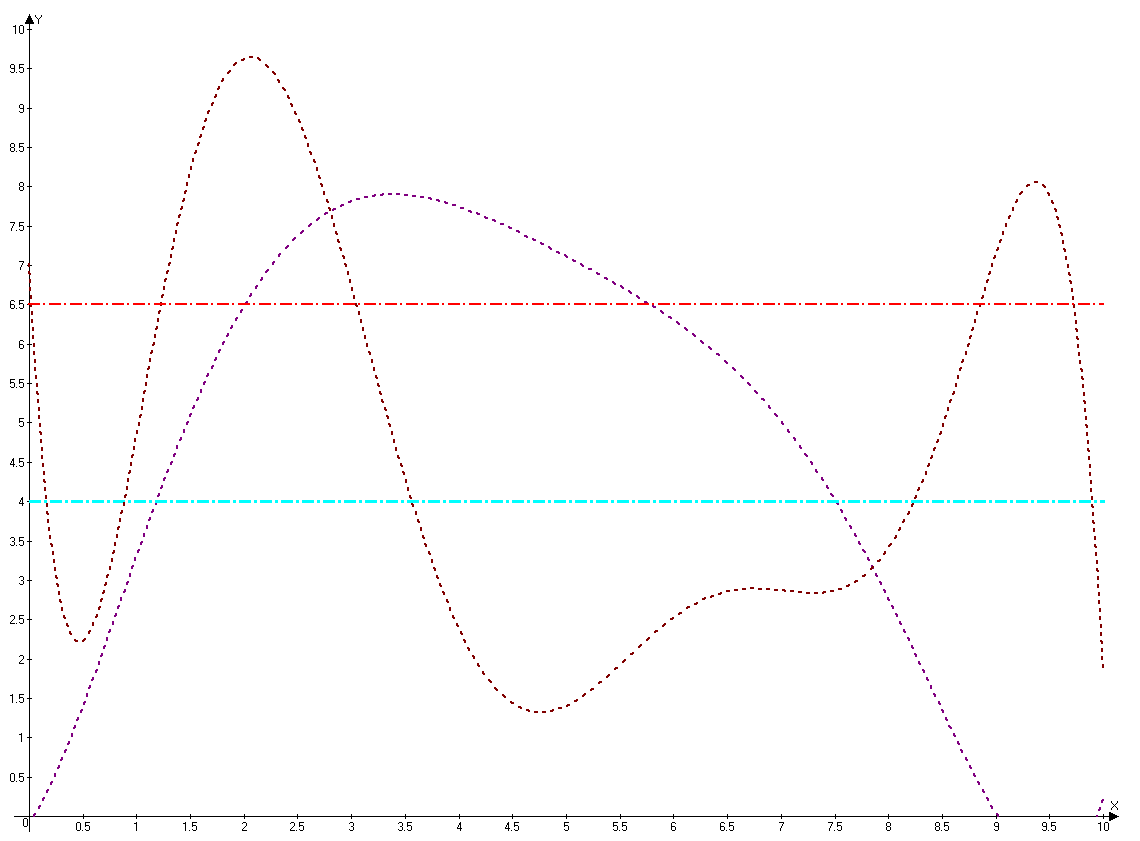
\includegraphics[width=1\linewidth]{MadMax-interpol.png}}
	\caption{Эскиз возможной интерполяции в ходе алгоритма позиционирования. Вертикальная ось --- уровень сигнала, горизонтальная --- координата. Штрихпунктирными линиями обозначены уровни фактически принятых сигналов от двух базовых станций (поскольку их координаты неизвестны, изображены на всём протяжении маршрута), штриховыми --- функции, интерполирующие имеющиеся в базе данных замеры.}
	\label{fig:madmax-interpol}
\end{figure}

\subsection{Вычисление псевдоплотности вероятности}

Одним из ключевых достижений данной работы является введение и применение для позиционирования функции псевдоплотности вероятности.

Определим функцию псевдоплотности вероятности как функцию двух переменных $P(f(x), y)$, где $y$ --- фактически измеренное значение RSSI в некоторой неизвестной точке, а $f(x)$ --- значение интерполяционного многочлена в известной точке $x$, удовлетворяющую следующим условиям:
\begin{enumerate}
	\item
		$\forall_{f(x), y}P(f(x), y)\in(0,1]$
	\item
		$\forall_{f(x), y}f(x) = y\Leftrightarrow{}P(f(x),y) = 1$
	\item
		$\lim\limits_{|f(x)-y|\to\infty}P(f(x),y) = 0$
\end{enumerate}

Функция, удовлетворяющая данным критериям, будет обладать следующим свойством: в любой точке маршрута, чем более фактический замер похож на значением многочлена в данной точке, тем ближе эта функция к 1, а чем дальше --- к 0. Этим свойством данная функция похожа на Байесовское понимание вероятности, а потому названа псевдоплотностью вероятности. Более того, также аналогично Байесовской вероятности, умножение двух таких функций, вычисленных для разных базовых станций, позволяет одновременно сравнивать похожесть по двум параметрам. За счёт того, что операцией, связывающей две псевдоплотности вероятности, является не сложение, как в функции расстояния Махаланобиса (пункт \ref{subsec:mahalanobis} на странице \pageref{subsec:mahalanobis}), а умножение, как в Байесовском классификаторе (пункт \ref{subsec:bayes} на странице \pageref{subsec:bayes}), все выбросы, если только не случится так, что в результате флуктуаций сигнал сразу от нескольких станций станет напоминать другую точку, взаимно уничтожаются.

\begin{figure}[H]
	\center{
		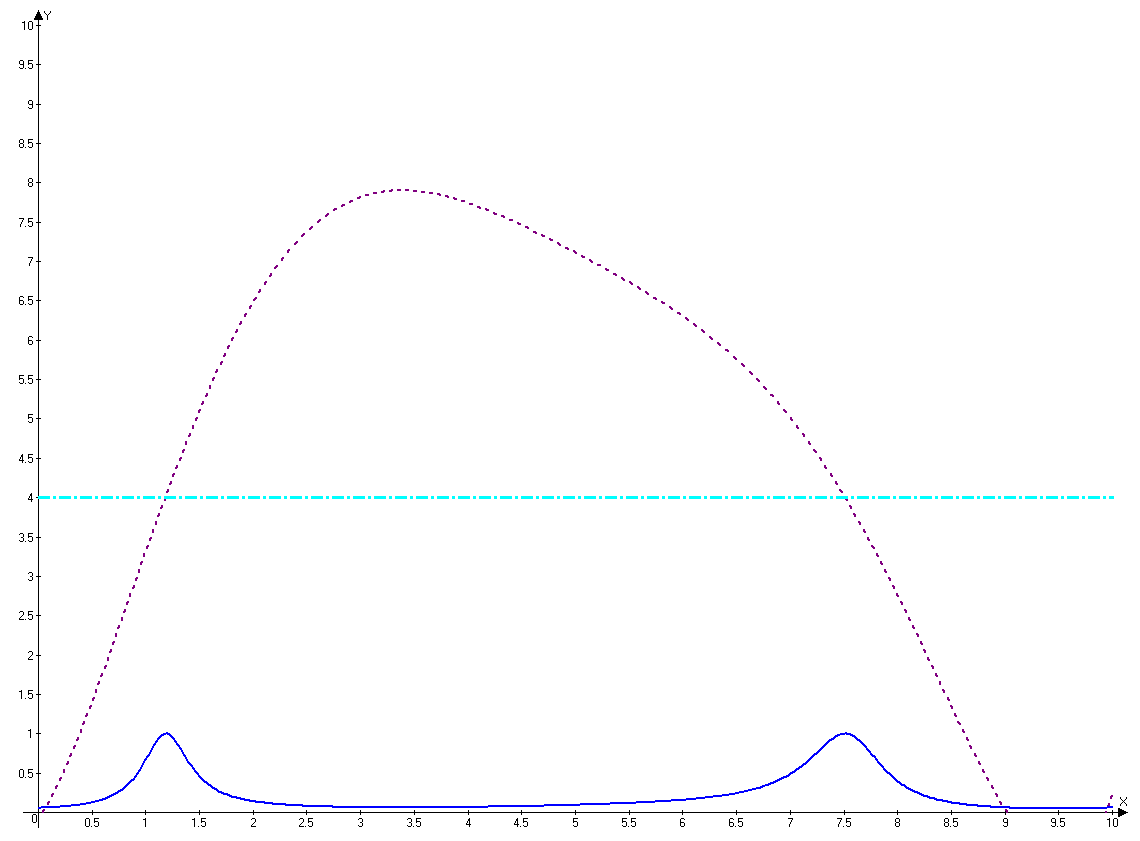
\includegraphics[width=0.7\linewidth]{MadMax-metr-1.png}
		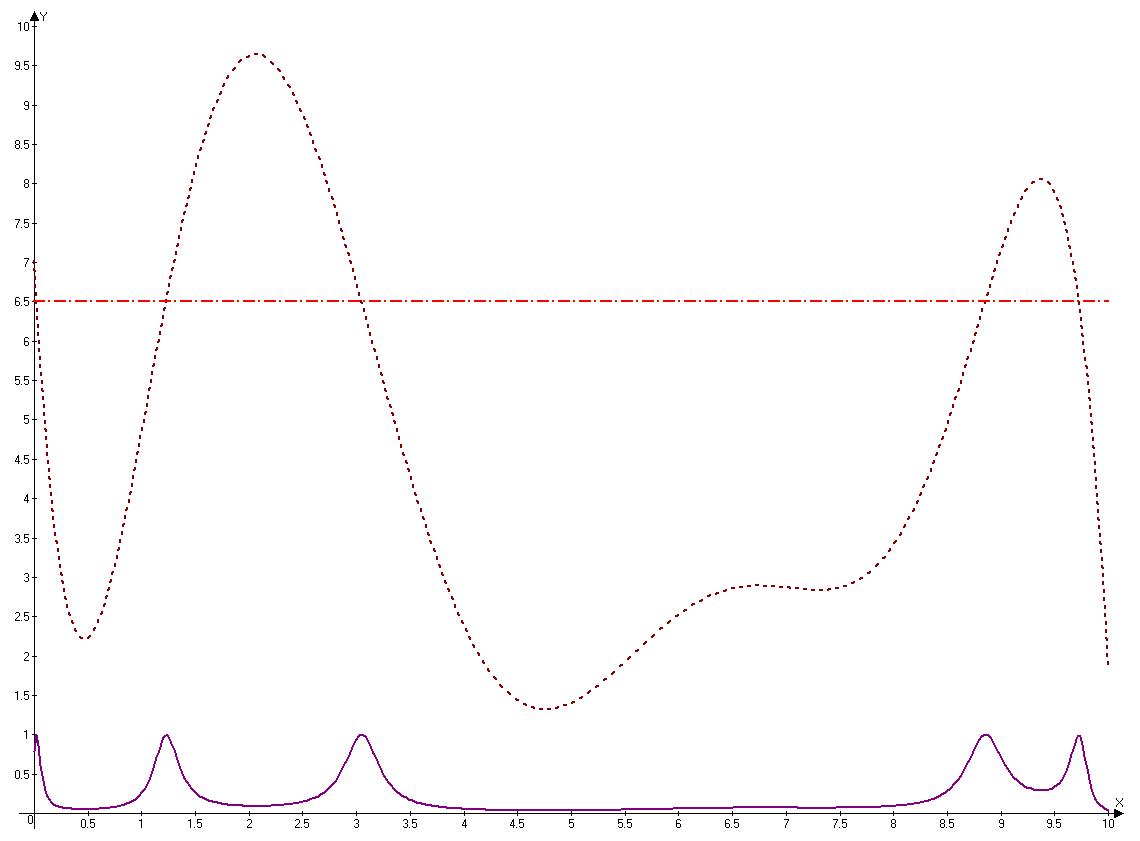
\includegraphics[width=0.7\linewidth]{MadMax-metr-2.png}
	}
	\caption{Эскиз процесса расчёта псевдоплотности вероятности для двух базовых станций. Горизонтальная ось --- расстояние, вертикальная --- RSSI и значение псевдоплотности (не в масштабе). Штрихпунктирная линия --- фактически измеренные значения RSSI, штриховая --- интерполяционный многочлен, сплошная --- значение псевдоплотности.}
	\label{fig:pseudop-draft}
\end{figure}

Отличает такую функцию от настоящей плотности вероятности следующее:
\begin{enumerate}
	\item
		Она может точно достигать значения 1, а не только приближаться к нему;
	\item
		Не требуется, а потому не гарантируется то, что интеграл этой функции по всей области определения равен 1;
	\item
		Даже если нормировать интеграл этой функции на 1, не гарантируется, что интеграл по некоторому участку действительно в точности равен частотной вероятности нахождения там устройства, хотя в Байесовском понимании она отражает степень уверенности в том, что устройство именно там.
\end{enumerate}

Вычисление истинной плотности вероятности не требуется, потому что для работы алгоритма её не нужно интегрировать, а только умножать и искать аргумент максимального значения. А в отношении этих свойств, данная функция сохраняет свойства, присущие плотности вероятности.

Отказ от возможности интегрирования, с другой стороны, позволяет ограничиться очень простым видом функции псевдоплотности вероятности, таким как \ref{eq:pseudop}.
\begin{equation}
	P(f(x), y) = \frac{1}{1+(f(x)-y)^2}
	\label{eq:pseudop}
\end{equation}

Эскиз процесса вычисления псевдоплотности вероятности показан на рис. \ref{fig:pseudop-draft}.

\subsection{Вычисление ответа}

\begin{figure}[H]
	\center{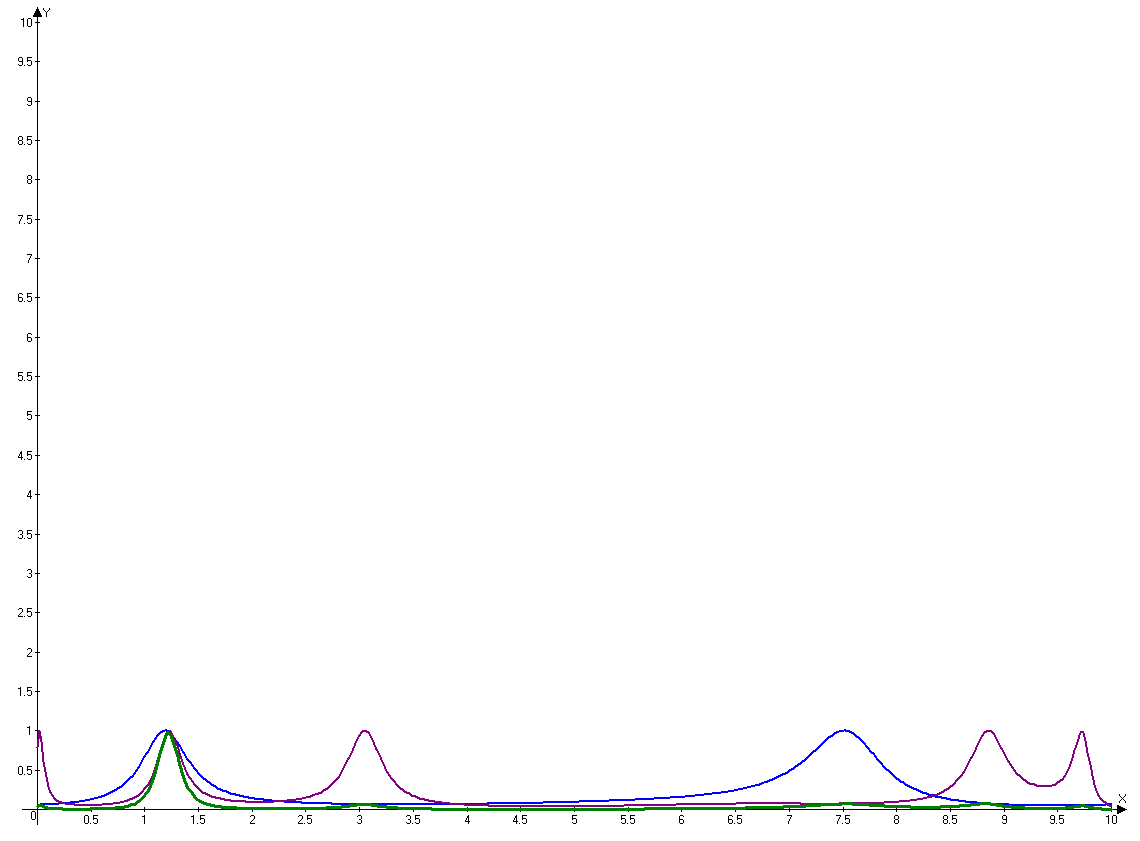
\includegraphics[width=1\linewidth]{MadMax-metr-common.png}}
	\caption{Эскиз произведения функций псевдоплотности для нескольких базовых станций. Горизонтальная ось --- точки на маршруте, вертикальная --- значения псевдоплотности. Результирующая псевдоплотность имеет всего один хорошо выраженный глобальный максимум между координатами 1 и 1,5.}
	\label{fig:total-pseudop-draft}
\end{figure}

После расчёта значений псевдоплотности вероятности для каждой базовой станции, процесс позиционирования сводится к их перемножению и поиску аргумента глобального максимума. Эскиз этого процесса показан на рис. \ref{fig:total-pseudop-draft}.

\section{Мобильное приложение}
Для ОС Android, выполняющейся на устройстве, оборудованном модулями GPS и GSM, а также предоставляющем доступ в интернет, требуется написать приложение, получающее данные об RSSI видимых базовых станций и своём местоположении, после чего передающее их на сервер.

\subsection{Протокол передачи данных}
Собранные данные передаются по протоколу UDP на сервер, будучи записанными в формате JSON в сообщения следующего вида:


\lstset{language=Python}
\begin{lstlisting}
{
	"GSM":{
		"cellcount":2, 
		"cells":[
				{
					"CID":11531, 
					"Psc":-1,
					"RSSI":26,
					"type":"EDGE"
				}, 
				{
					"CID":32779,
					"Psc":-1,
					"RSSI":22,
					"type":"EDGE"
				}
			]
		},
	"GPS": {
			"lng":37.64814019203186,
			"ltd":55.75437605381012,
			"acc":24.0
		}
}
\end{lstlisting}

Значения содержимого полей описаны в таблице \ref{tab:json-raw-format}.
\begin{table}
	\caption{\label{tab:json-raw-format}Значения полей пакета в формате JSON, передаваемого от мобильного устройства на сервер.}
	\begin{center}
		\begin{tabular}{|p{0.2\linewidth}|p{0.2\linewidth}|p{0.5\linewidth}|}
			\hline
			Поле & Тип & Значение \\
			\hline
			GSM & Объект & Набор данных о видимых базовых станций \\
			\hline
			cellcount & Число & Количество станций, передаваемых в данном пакете \\
			\hline
			cells & Массив & Набор объектов, каждый из которых соответствует одной базовой станции \\
			\hline
			CID & Число & Уникальный идентификатор базовой станции, 2 байта \\
			\hline
			Psc & Число & Зарезервировано для сетей 3G \\
			\hline
			RSSI & Число & Уровень принятого сигнала в asu\\
			\hline
			type & Строка & Тип соединения. Возможные значения: <<GPRS>>, <<EDGE>>, <<UMTS>>, <<UNKNOWN>> \\
			\hline
			GPS & Объект & Набор данных спутниковой навигации \\
			\hline
			lng & Число & Долгота в градусах \\
			\hline
			ltd & Число & Широта в градусах \\
			\hline
			acc & Число & Погрешность позиционирования в метрах \\
			\hline
		\end{tabular}
	\end{center}
\end{table}

\subsection{Интерфейсы}

Особенностью программирования под Android SDK является тот факт, что в программе нет аналога функции или метода Main из многих популярных языков программирования. Вся программа состоит из обработчиков различных событий, происходящих в графическом интерфейсе или внутри ОС Android. Запустить код, не зависящий от обработчиков, можно только создав отдельный поток во время обработки одного из событий в главном.

В связи с этим, приложение можно полностью описать через его взаимодействие с иными компонентами.

\subsubsection{Графический интерфейс}
\begin{figure}[h]
	\center{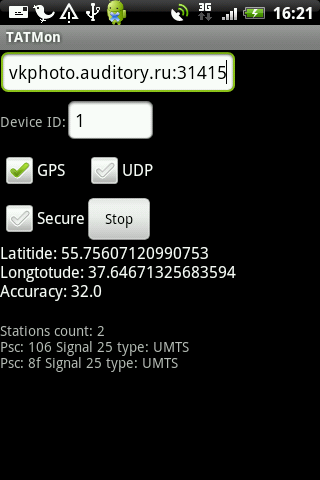
\includegraphics[width=0.5\linewidth]{TATMon-android.png}}
	\caption{Графический интерфейс написанного мобильного приложения, запущенного на телефоне HTC Hero под управлением Android 2.2.}
	\label{fig:tatmon-android}
\end{figure}
Графический интерфейс приложения изображён на рис. \ref{fig:tatmon-android}.
По нажатию кнопки <<Start>>/<<Stop>> начинается или приостанавливается работа фонового потока, обеспечивающего сбор и передачу данных. Этому потоку передаётся адрес и порт, по которому нужно посылать данные, значение флага GPS, определяющего, надо ли передавать данные спутникового позиционирования, или же только уровни сигнала. При неустановленном флаге UDP, фоновый поток не передаёт данные в сеть, а только возвращает их потоку графического интерфейса, который при наступлении такого события как приход сообщения о фонового, обновляет отображаемый список.

Поле Device ID и флаг Secure в описываемой версии не используются.

\subsubsection{Данные об уровнях сигнала}
Информацию об уровнях сигналов видимых базовых станций предоставляется объект класса TelephonyManager, который инстанциируется операционной системой в главном потоке. Информацию он предоставляет через синхронный вызов функции, возвращающей ответ. В связи с этим, обработка этих данных ведётся в фоновом потоке.

\subsubsection{Данные спутниковой навигации}
Данные же GPS поступают асинхронно. При включённом модуле GPS операционная система сама отслеживает факт измерения координат, и создаёт событие обновления, которое можно обработать. Эта обработка осуществляется в главном потоке, после чего её результаты передаются фоновому.

\subsubsection{Взаимодействие с сетью}
Передача данных через UDP осуществляется синхронным вызовом функции, а потому вместе с обработкой данных об уровнях сигнала вынесена в фоновый поток.

\section{Серверная часть}
Сервер, в целом, осуществляет две задачи: приём и обработка поступающих данных и передача результатов работы клиенту. Разница между этими процессами заключается в том, что приходящие по UDP данные обрабатываются синхронно, а передача клиенту по TCP --- асинхронно. В связи с этим, сервер работает в два потока, передача данных между которыми осуществляется через библиотечный класс Queue. Схема этого процесса изображена на рис. \ref{fig:server-threads}.

\begin{figure}[h]
	\center{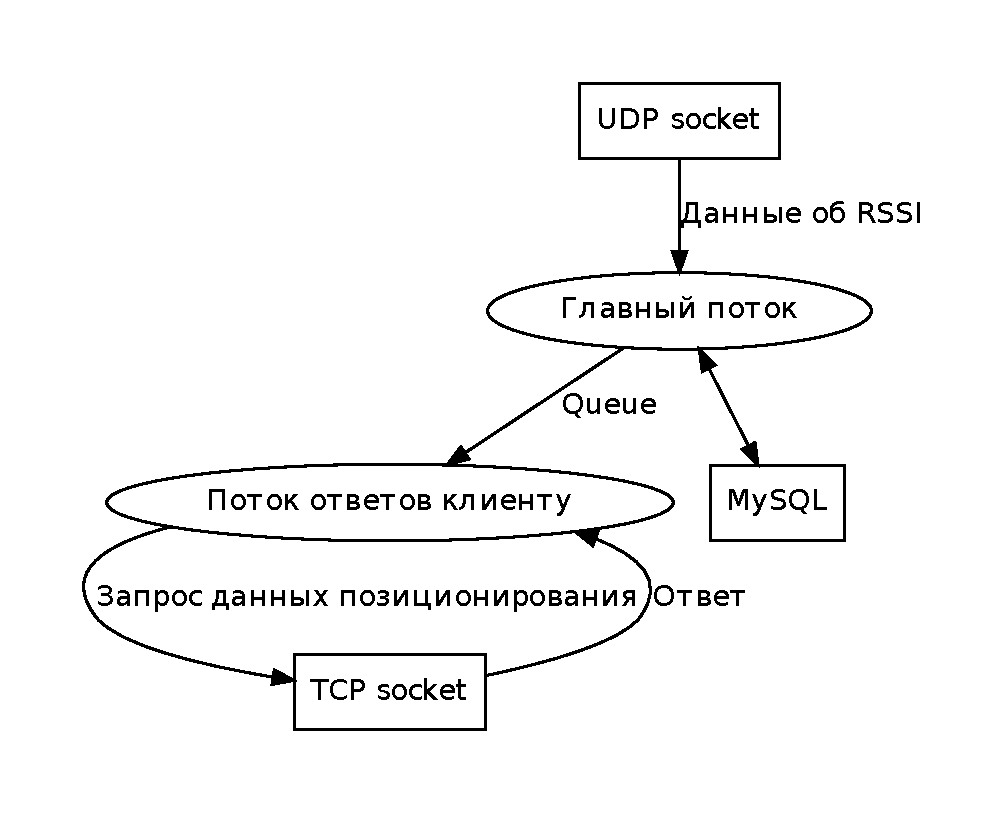
\includegraphics[width=1\linewidth]{server-threads.pdf}}
	\caption{Взаимодействие между потоками сервера (эллипсы) и внешними интерфейсами (прямоугольники).}
	\label{fig:server-threads}
\end{figure}

Сервер может работать в двух режимах --- сбор данных и тестирование позиционирования. Часть классов и модулей является общей для обоих режимов, часть --- специфичной для позиционирования. Начнём, поэтому, с описания режима сбора данных, в рамках описания которого опишем и общие классы.

\subsection{Режим сбора данных}
\begin{figure}[h]
	\center{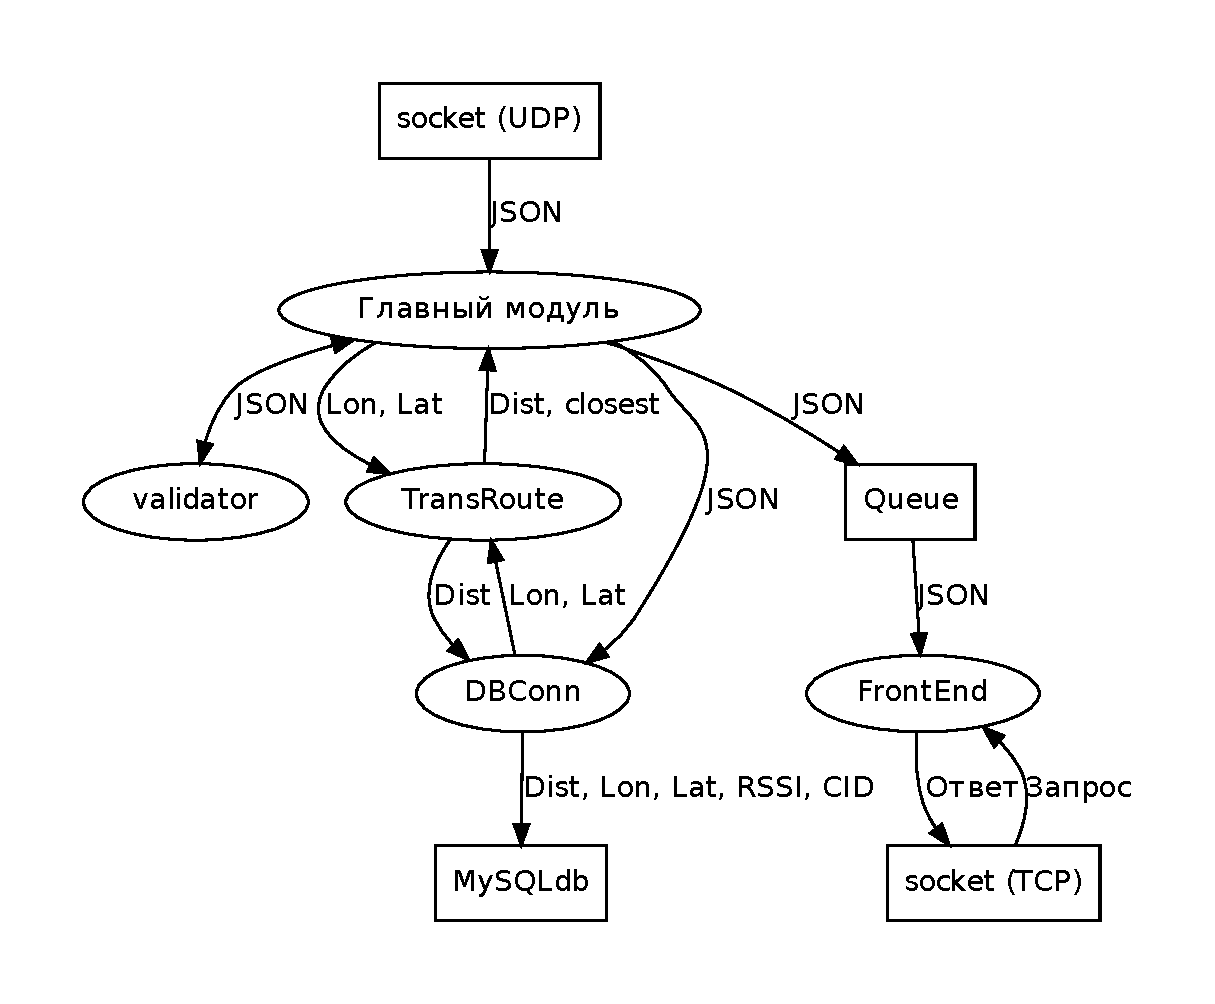
\includegraphics[width=1\linewidth]{server-collect-dataflow.pdf}}
	\caption{Потоки данных между классами сервера (эллипсы) и внешними интерфейсами (прямоугольники) в режиме сбора данных.}
	\label{fig:server-collect-dataflow}
\end{figure}
Общая схема направлений потоков данных в режиме сбора данных изображена на рис. \ref{fig:server-collect-dataflow}. Не отображено преобразование данных в формате JSON во внутренне представление Python, но поскольку и прямое, и обратное преобразование осуществляются каждое одной функцией, их в описании потоков опускаем. Рассмотрим теперь подробнее каждый из классов и модулей, участвующих в обработке данных.

\subsubsection{Проверка входящих данных}
Модуль {\bf validator} содержит единственную функцию с таким же названием, осуществляющую проверку входящих данных на наличие и корректные значения всех полей, описанных в \ref{tab:json-raw-format}. В случае, если находится несоответствие, функция возвращает специальное значение None, получение которого обрабатывается, в противном случае --- переданный объект.

\subsubsection{Преобразование координат}
\label{subsubsec:transroute}
Класс {\bf TransRoute} осуществляет три операции: преобразование пары широта/долгота в расстояние от начала маршрута, обратно --- расстояние в широту и долготу, а также находит точку на маршруте, ближайшую к переданной.

В прототипе системы была реализована обработка единственного маршрута, представляющего собой прямую линию с известными координатами начала и конца. Нетривиальной в таком случае является только одна задача: поиск точки на маршруте, ближайшей к данной. Необходимость её решения вызвана тем, что GPS сам обладает некоторой погрешностью, и может возвращать координаты не строго на маршруте, а немного сбоку от него, поэтому сначала полученную точку надо найти её проекцию на маршрут.

Координаты начала и конца маршрута передаются в конструктор класса, сам класс имеет следующие методы:

\begin{itemize}
	\item
		{\bf closest} --- принимает описание широты и долготы точки в формате JSON, возвращает кортеж из двух координат её проекции на маршрут;
	\item
		{\bf point\_to\_dist} --- принимает описание широты и долготы точки в формате JSON, возвращает число --- расстояние от начала маршрута до проекции переданной точки на него. Расстояние имеет знак, если выйти за границу маршрута со стороны начала, будет также корректным расстоянием по модулю, но отрицательным;
	\item
		{\bf dist\_to\_longlat} --- принимает расстояние от начала маршрута до искомой точки, возвращает её географические координаты.
\end{itemize}

\subsubsection{Взаимодействие с базой данных}
Все запросы к базе данных осуществляются через класс {\bf DBConn}. Подробное описание базы данных находится в подразделе \ref{sec:server-db}, а здесь дано общее описание осуществляемых запросов:
\begin{itemize}
	\item
		{\bf save\_netdata} --- принимает объект JSON с данными о GPS и RSSI, записывает их в базу данных как в виде географических координат, так и в виде точек на маршруте; для преобразования использует класс TransRoute;
	\item
		{\bf avg\_rssi} --- принимает CellID, возвращает среднее значение RSSI по всем точкам;
	\item
		{\bf all\_cells} --- возвращает список из всех CellID, данные о которых имеются в базе;
	\item
		{\bf samples\_by\_sell} --- принимает CellID, возвращает все результаты замеров для неё.
\end{itemize}

\subsubsection{Взаимодействие с клиентами}
\label{subsubsec:server-collect-frontend}
Класс {\bf{}FrontEnd} наследует библиотечный класс {\bf{}threading.Thread} и перегружает единственный метод {\bf{}run}, выполняющийся в отдельном потоке. Метода run, будучи запущенным, открывает сокет для входящих соединений от клиентов, после чего в бесконечном цикле ждёт их. После установки соединения, во вложенном бесконечном цикле пытается считать сообщение из очереди, идущей от главного потока, и если это удалось, посылает его в сокет. При обрыве соединения вложенный бесконечный цикл завершается с исключением, которое обрабатывается внешним, после чего последний снова ожидает соединений.

Передача данных начинается сразу по мере установки соединения клиентом, без ожидание запросов с его стороны. Передаются данные в формате JSON следующего вида:
\begin{lstlisting}
{
	"GPSerrm": 5.8398814870603832,
	"Route": {
		"lng": 37.647922706087265,
		"dstm": 260.0450561256485,
		"dst": 0.0023370777009036913,
		"ltd": 55.754401640921643
	}, 
	"GPSerr": 5.2484200248492898e-05, 
	"GPS": {
		"lng": 55.75437605381012,
		"ltd": 37.647968530654907
		}
}
\end{lstlisting}

Значения полей описаны в таблице \ref{tab:json-collect-format}.

\begin{table}
	\caption{\label{tab:json-collect-format}Значения полей пакета в формате JSON, передаваемого от сервера в режиме сбора данных клиентам.}
	\begin{center}
		\begin{tabular}{|p{0.2\linewidth}|p{0.2\linewidth}|p{0.5\linewidth}|}
			\hline
			Поле & Тип & Значение \\
			\hline
			GPSerrm & Число & Расстояние между точкой и её проекцией на маршрут в метрах \\
			\hline
			Route & Объект & Информация о точке на маршруте \\
			\hline
			lng & Число & Долгота в градусах \\
			\hline
			ltd & Число & Широта в градусах \\
			\hline
			dst & Число & Расстояние от начала маршрута в градусах \\
			\hline
			dstm & Число & Расстояние от начала маршрута в метрах \\
			\hline
			GPSerr & Число & Расстояние между точкой и её проекцией на маршрут в градусах \\
			\hline
		\end{tabular}
	\end{center}
\end{table}

\subsubsection{Главный модуль}
\label{subsubsec:collect-data-main}
Алгоритм работы главного модуля в режиме сбора данных состоит из инициализации всех классов, открытия UDP-сокета для входящих датаграмм от мобильных устройств и перехода в следующий бесконечный цикл:
\begin{enumerate}
	\item
		Принятие сообщения;
	\item
		Проверка сообщения модулем validate;
	\item
		Запись сообщения в базу данных модулем DBConn;
	\item
		Вычисление проекции принятой точки на маршрут, её расстояния от начала маршрута, расстояния между исходной точкой и её проекцией;
	\item
		Запись посчитанных значений в формат JSON и отправка в очередь потока FrontEnd.
\end{enumerate}

\subsection{Режим позиционирования}
Режим позиционирования отличается от режима сбора данных тем, что реакцией на приход сообщения от мобильного устройства является не помещение этой информации в базу данных, а позиционирование на основе собранных данных, проверка качества работы на основе пришедших данных спутникового позиционирования и отправка этих данных клиенту. Соответственно, в архитектуру добавляются классы, обеспечивающие процесс позиционирования. Общий вид потоков данных в режиме позиционирования изображён на рис. \ref{fig:server-perform-dataflow}.

\begin{figure}[h]
	\center{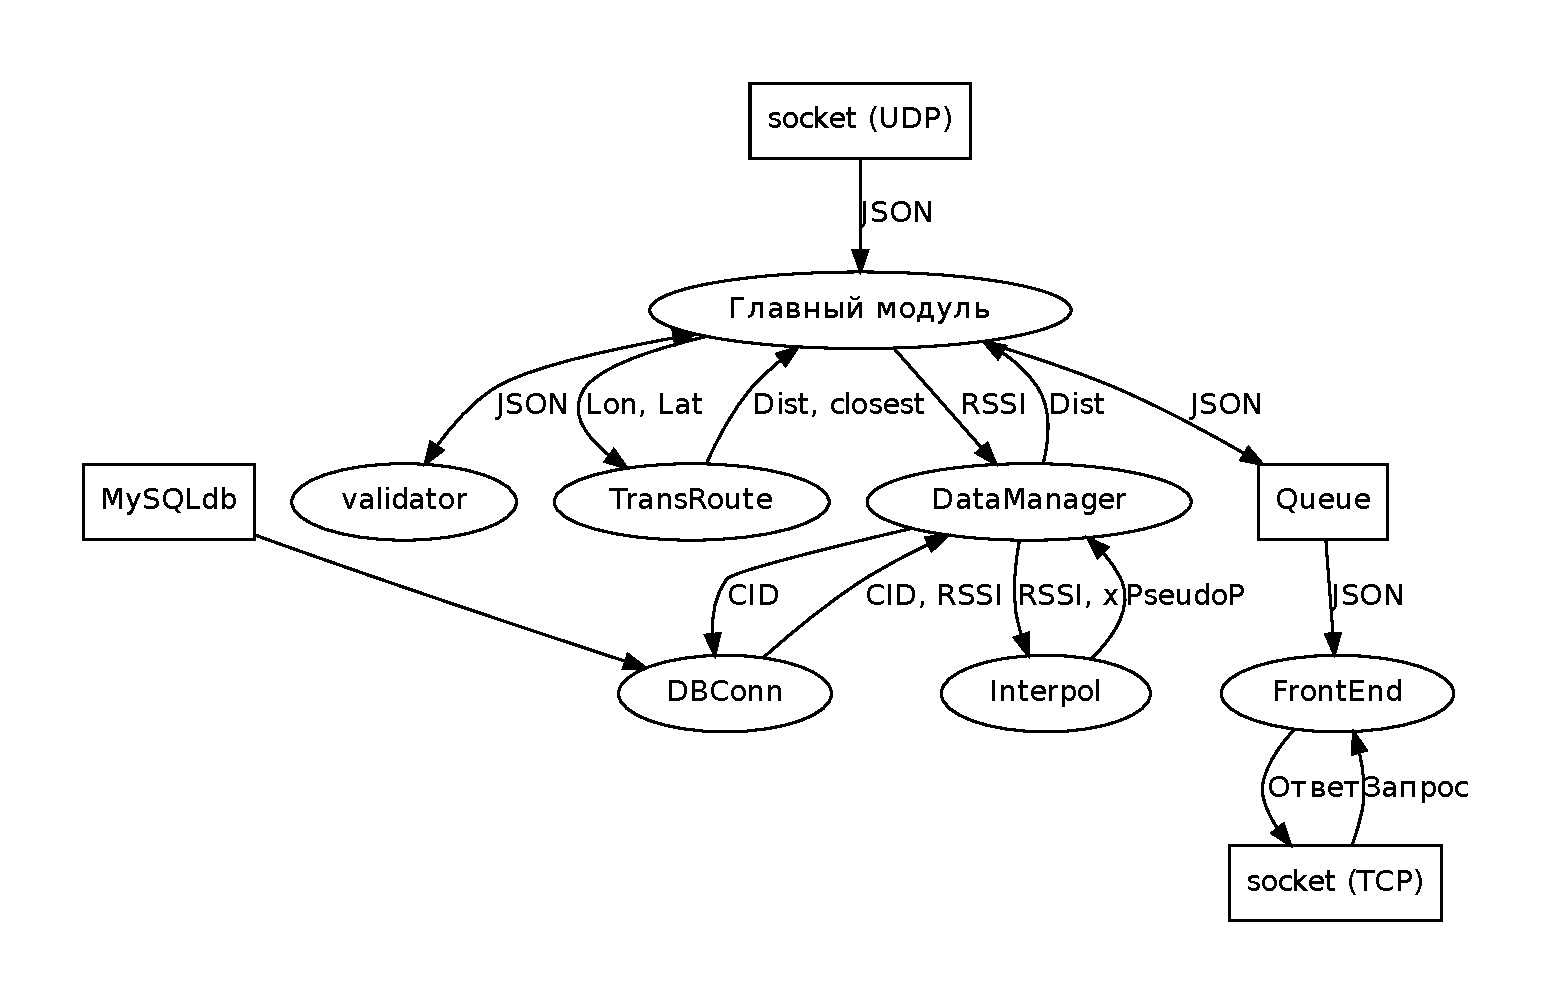
\includegraphics[width=1\linewidth]{server-perform-dataflow.pdf}}
	\caption{Потоки данных между классами сервера (эллипсы) и внешними интерфейсами (прямоугольники) в режиме позиционирования.}
	\label{fig:server-perform-dataflow}
\end{figure}

\subsubsection{Интерполяция и псевдоплотность}
Класс {\bf{}Interpol} предоставляет набор функций для построения интерполирующего многочлена, вычисления его значений для конкретных точек, а также вычисления псевдоплотности вероятности для данной точки на маршруте и данного уровня сигнала. Один экземпляр данного класса описывает перечисленные сущности для одной базовой станции.

Код этого класса, как реализующего основу разработанного математического метода, приводится целиком:

\lstset{language=Python}
\begin{lstlisting}
#-*- coding: utf8 -*-
import numpy
import numpy.linalg

import sys
class Interpol(object):
	def __init__(self, order=10):
		self.order = order
		self.theta = [0]*(self.order+1)

	def create_vars(self, data):
		l = len(data)
		print l
		self.X = numpy.empty([l, self.order+1])
		self.Y = numpy.empty([l, 1])
		try:
			for j in xrange(l):
				for i in xrange(0,self.order+1):
					self.X[j][i] =\
						data[j][0]**i
				self.Y[j][0] = data[j][1]
		except Exception as e:
			print e
			print "i:", i, "j:", j
			print "order:", self.order
			print "data[j]:", data[j]
			print "self.X[j][i]", self.X[j][i]
			print "self.Y[j][0]:", self.Y[j][0]
			sys.exit(0)

	def solve_theta(self):
		self.theta = numpy.transpose(self.X)
		self.theta = numpy.dot(self.theta, self.X)
		self.theta = numpy.linalg.pinv(self.theta)
		self.theta = numpy.dot(self.theta,\
				numpy.transpose(self.X))
		self.theta = numpy.dot(self.theta, self.Y)

	def value(self, x):
		res = 0
		for i in xrange(0, self.order+1):
			res += self.theta[i] * x**i
		return res


	def pseudop(self, x, y):
		return 1.0/(1.0+(self.value(x)-float(y))**2)
\end{lstlisting}

Данный класс использует библиотеку NumPy для быстрых вычислений, предоставляющую интерфейс к ряду математических библиотек, конкретный набор которых зависит от платформы, под GNU/Linux используется GNU Scientific Library\cite{gsl}. Вычисления, даже будучи по своей природе векторными, в случае применения GSL, осуществляются в один поток, однако для данной задачи этого оказалось достаточно.

Конструктор класса {\bf{}\_\_init\_\_} в качестве необязательного аргумента принимает максимальную степень требуемого интерполяционного многочлена, после чего сохраняет её значение в поле order и создаёт массив theta для его коэффициентов.

Два метода должны быть вызваны в обязательном порядке:
\begin{enumerate}
	\item
		{\bf{}create\_vars} --- этот метод в качестве аргумента принимает список data, состоящий из пар $<Dist, RSSI>$ и содержащий все ранее измеренные значения RSSI исследуемой базовой станции в известных точках Dist:
		\begin{equation}
			data = \begin{pmatrix}
				Dist_0 & RSSI_0 \\
				Dist_1 & RSSI_1 \\
				\vdots & \vdots \\
     Dist_{len(data)-1} & RSSI_{len(data)-1}
			\end{pmatrix}
			\label{eq:data-create-vars}
		\end{equation}
		Результатом работы данного метода является запись в поля класса двух массивов: массива self.X, состоящего из векторов $<1, Dist_i, Dist_i^2, ... Dist_i^{order}>$, и массива self.Y, состоящего из значений RSSI, расположенных в том же порядке, что соответствующие им значения $Dist_i$ в массиве self.X:
		\begin{equation}
			self.X = \begin{pmatrix}
				1 & Dist_0 & Dist_0^2 & \cdots & Dist_0^{order} \\
				1 & Dist_1 & Dist_1^2 & \cdots & Dist_1^{order} \\
      \vdots & \vdots & \vdots & \vdots & \vdots \\
				       1 & Dist_{len(data)-1} & Dist_{len(data)-1}^2 & \cdots & Dist_{len(data)-1}^{order}
			\end{pmatrix}
			\label{eq:self-x-create-vars}
		\end{equation}
		\begin{equation}
			self.Y = \begin{pmatrix}
				RSSI_0 \\
				RSSI_1 \\
				\vdots \\
				RSSI_{len(data)-1}
			\end{pmatrix}
			\label{eq:self-y-create-vars}
		\end{equation}
	\item
		{\bf{}solve\_theta} --- результатом вызова этого метода является нахождение коэффициентов интерполяционного многочлена по методу нормальных уравнений и запись их в массив self.theta:
		\begin{equation}
			self.theta = (self.X^\intercal \cdot self.X)^{+} \cdot self.X^\intercal \cdot self.Y
			\label{eq:solve-theta}
		\end{equation}
		Отметим, что в ходе решения используется не обычная инверсия, а нахождение псевдообратной матрицы, что позволяет сохранить работоспособность системы даже в случае, когда система неразрешима в рамках обычного метода нормальных уравнений.
\end{enumerate}

После того, как были вызваны эти методы, становится доступным вызов метода {\bf{}value}, возвращающего значение интерполяционного многочлена в переданной точке, и метода {\bf{}pseudop}, для заданной точки и заданного уровня RSSI возвращающего значение псевдоплотности вероятности.

\subsubsection{Результирующая псевдоплотность и позиционирование}

Класс {\bf{}DataManager} отвечает за хранение коллекции экземпляров класса Interpol, соответствующих различным базовым станциям, и использование их для позиционирования устройств. В прототипе системы приняты следующие соглашения:

\begin{enumerate}
	\item
		Интерполяционные многочлены строятся при инициализации сервера в режиме позиционирования, сразу для всех имеющихся в базе данных CellID;
	\item
		Одновременно сервер работает только в одном из режимов, а потому во время работы в режиме позиционирования, состояние базы данных измениться не может, и перестраивать многочлены гарантированно не потребуется;
	\item
		Весь процесс выборки данных из базы, соответственно, происходит только во время инициализации, после чего в течение всего времени работы сервера интерполяционные многочлены хранятся в оперативной памяти.
\end{enumerate}

С учётом этих соглашений, рассмотрим работу класса DataManager. При вызове конструктора класса создаётся подключение к базе данных через класс DBConn, после чего в обязательном порядке должны быть вызваны следующие методы:

\begin{enumerate}
	\item
		{\bf{}fetch\_cells} --- этот метод передаёт классу DBConn запрос на получение списка всех CellID, имеющихся в базе данных, после чего записывает результат в своё поле self.cells;
	\item
		{\bf{}build\_interpols} --- для каждого из полученных CellID, этот метод передаёт классу DBConn запрос на получение всех результатов измерений, связанных с данной базовой станцией, после чего создаёт объект класса Interpol, у которого вызывает метод create\_vars со списком измерений в качестве аргумента, после чего вызывает метод solve\_theta. Полученный объект, готовый к использованию для вычисления псевдоплотности, помещается в ассоциативный массив self.cellfuncs с CellID в качестве индекса.
\end{enumerate}

После вызова этих методов, становятся доступными следующие:
\begin{itemize}
	\item
		{\bf{}total\_pseudop} --- для заданного списка $<CID, RSSI>$ и заданной точки на маршруте, вычисляет значения псевдоплотности, после чего перемножает их между собой и возвращает результат.
	\item
		{\bf{}position} --- для заданного списка $<CID, RSSI>$ перебирает все возможные значения x и возвращает то, для которого значение общей псевдоплотности было максимальным. Для работы прототипа системы, даже такого простого метода поиска максимума оказалось достаточно, хотя, в случае реализации для промышленного применения, его стоит заменить на более эффективный.
\end{itemize}

\subsubsection{Главный модуль}
\label{subsubsec:server-perform-main}
Алгоритм работы главного модуля в режиме позиционирования схож с алгоритмом в режиме сбора данных (см. подпункт \ref{subsubsec:collect-data-main}), а отличается тем, что в начале работы, среди прочих, инициализируется класс DataManager, а бесконечный цикл состоит из следующих этапов:

\begin{enumerate}
	\item
		Приём данных от мобильного устройства;
	\item
		Валидация принятых данных;
	\item
		Позиционирование по данным GSM с помощью класса DataManager;
	\item
		Перевод координат полученной точки из одного числа --- расстояния от начала маршрута --- в пару широта/долгота;
	\item
		Сравнение полученных данных с данными GPS, также принятыми от мобильного устройства;
	\item
		Отправка всех вычисленных данных в формате JSON в очередь класса FrontEnd.
\end{enumerate}

Клиенту от сервера передаётся сообщение в формате JSON следующего вида:
\begin{lstlisting}
{
    "RouteGPS": {
        "dstd": 0.0033751292307418156, 
        "dstm": 375.73660822935375, 
        "fromtruem": 13.135102486978056, 
        "lng": 55.755307975824707, 
        "ltd": 37.648428777250331
    }, 
    "RouteGSM": {
        "dstm": 336.50000000000193, 
        "lng": 37.648256950398967, 
        "ltd": 55.755000247022828
    }, 
    "TrueGPS": {
        "acc": 8.0, 
        "lng": 55.755250453948975, 
        "ltd": 37.648531794548035
    }
}
\end{lstlisting}

Описание значения полей даны в таблице \ref{tab:json-perform-format}.

\begin{table}
	\caption{\label{tab:json-perform-format}Значения полей пакета в формате JSON, передаваемого от сервера в режиме позиционирования клиентам.}
	\begin{center}
		\begin{tabular}{|p{0.2\linewidth}|p{0.2\linewidth}|p{0.5\linewidth}|}
			\hline
			Поле & Тип & Значение \\
			\hline
			RouteGPS & Объект & Набор данных о проекции истинного положения устройства на маршрут \\
			\hline
			dsts & Число & Расстояние от начала маршрута до проекции положения в градусах \\
			\hline
			dstm & Число & Расстояние от начала маршрута до проекции положения в метрах \\
			\hline
			fromtruem & Число & Расстояние от истинного положения до его проекции на маршрут в метрах \\
			\hline
			lng & Число & Долгота в градусах \\
			\hline
			ltd & Число & Широта в градусах \\
			\hline
		   	RouteGSM & Объект & Набор данных о результатах позиционирования по сигналу GSM \\
			\hline
			TrueGPS & Объект & Набор данных об истинном положении мобильного устройства по данным спутниковой навигации \\
			\hline
			acc & Число & Погрешность GPS в метрах\\
			\hline
		\end{tabular}
	\end{center}
\end{table}

\section{База данных}
\label{sec:server-db}
Необходимость хранить данные об отношении между точками на маршруте и результатами измерений уровней сигнала в них, по определению, говорит о необходимости использования реляционной модели.

В разработанном прототипе системы используется простая база данных, состоящая из двух таблиц, хранящих результаты измерений RSSI в различных точках маршрута для различных базовых станций. Никакие другие другие данные длительного хранения не требуют.

Имеющиеся таблицы объявлены следующим образом:

\lstset{language=SQL}
\begin{lstlisting}
CREATE TABLE IF NOT EXISTS raw_rssi_data (
	Longitude DOUBLE NOT NULL,
	Latitude DOUBLE NOT NULL,
	CellID INT NOT NULL,
	ObservedRSSI INT NOT NULL,
	Observations INT NOT NULL,
	PRIMARY KEY (Longitude, Latitude, CellID, ObservedRSSI),
	INDEX (CellID)
) ENGINE=InnoDB;

CREATE TABLE IF NOT EXISTS route_rssi_data (
	Route INT NOT NULL,
	Distance DOUBLE NOT NULL,
	CellID INT NOT NULL,
	ObservedRSSI INT NOT NULL,
	Observations INT NOT NULL,
	PRIMARY KEY (Route, Distance, CellID, ObservedRSSI),
	INDEX (CellID)
) ENGINE=InnoDB;
\end{lstlisting}

\begin{table}
	\caption{\label{tab:server-db}Значения столбцов в таблицах базы данных сервера}
	\begin{center}
		\begin{tabular}{|p{0.2\linewidth}|p{0.7\linewidth}|}
			\hline
			Столбец & Значение \\
			\hline
			Longitude & Долгота в градусах \\
			\hline
			Latitude & Широта в градусах \\
			\hline
			CellID & Уникальный идентификатор базовой станции, целое число \\
			\hline
			ObservedRSSI & Измеренное значение уровня сигнала от данной базовой станции в данной точке в asu\\
			\hline
			Observations & Количество раз, которое уровень сигнала от данной базовой станции принимал в данной точке данное значение\\
			\hline
			Distance & Расстояние от начала маршрута в градусах \\
			\hline
			Route & Номер маршрута, зарезервировано для дальнейшего развития \\
			\hline
		\end{tabular}
	\end{center}
\end{table}

Значения их столбцов описаны в таблице \ref{tab:server-db}. Видно, что имеющие таблицы дублируют друг друга. Такая архитектура была выбрана в связи с тем, что для работы сервера требуется только данные из таблицы route\_rssi\_data, ассоциация же результатов измерений с их истинным положением, а не его проекцией на маршрут, требуется только для целей сбора и анализа статистики. Таким образом, таблицу raw\_rssi\_data следует считать хранилищем отладочной информации, а реально используемой базой данных --- только route\_rssi\_data.

\subsection{Добавление информации в БД}
Хранение для каждой точки и каждой базовой станции не среднего результата всех замеров, а количества наблюдений для каждого из наблюдавшегося уровня по отдельности, по сути, представляет собой хранение распределения. Это позволяет однозначно восстановить все когда-либо сделанные замеры (что используется для увеличения множества, на котором строятся интерполяционные многочлены), при этом не перегружая базу уникальными идентификаторами для каждого наблюдения.

С другой стороны, это усложняет добавление информации о новом наблюдении в базу. Оно разделяется на два случая:
\begin{enumerate}
	\item
		Если для измеренной тройки $<Distance, CellID, ObservedRSSI>$ в таблице уже имеется строка с точно такими же значениями, требуется увеличить на 1 значение ячейки Observations этой строки;
	\item
		Если же таких значений нет, подобную строку надо добавить в таблицу, установив значение ячейки Observations в 1.
\end{enumerate}

Поскольку MySQL не поддерживает триггеры типа <<INSTEAD OF INSERT>>\cite{triggersyntax}, осуществляет эту операцию сервер по следующему алгоритму:
\begin{enumerate}
	\item
		Начало транзакции;
	\item
		Запрос вида: <<SELECT Longitude, Latitude, CellID, ObservedRSSI FROM\\* raw\_rssi\_data WHERE Longitude = \%4.15f AND Latitude = \%4.15f AND CellID = \%d AND ObservedRSSI = \%d>>;
	\item
		\begin{itemize}
			\item
				Если результат запроса пустой --- запрос вида: <<INSERT INTO\\* raw\_rssi\_data(Longitude, Latitude, CellID, ObservedRSSI, Observations) VALUES (\%4.15f, \%4.15f, \%d, \%d, \%d)>>;
			\item
				Иначе --- запрос вида: <<UPDATE raw\_rssi\_data SET Observations = Observations + 1 WHERE Longitude = \%4.15f AND Latitude = \%4.15f AND CellID = \%d AND ObservedRSSI = \%d>>;
		\end{itemize}
	\item
		Конец транзакции.
\end{enumerate}

\section{Клиентская часть}
Несмотря на то, что основная информация о работе сервера собиралась с помощью текстовых журналов, для контроля его работы в реальном времени был написан графический клиент на языке Python с использованием библиотеки Pygame.

\begin{figure}[h]
	\center{
		\begin{subfigure}[b]{0.7\textwidth}
			\center{
				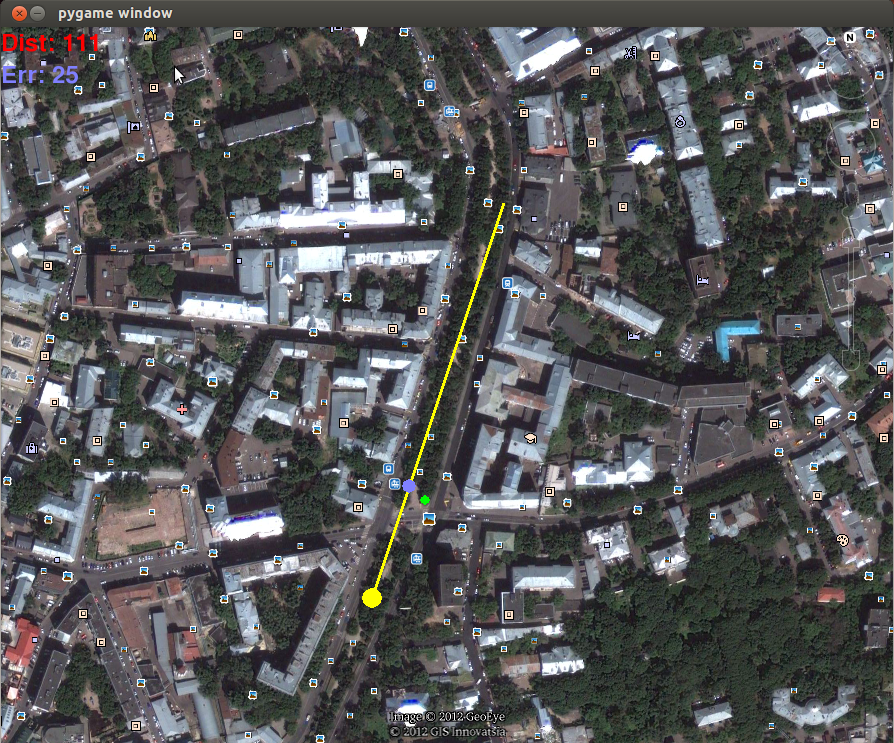
\includegraphics[width=\textwidth]{gfront-gps-mode.png}
				\caption{Сбор данных}
			}
			\label{subfig:gfront-gps-mode}
		\end{subfigure}
	
		\begin{subfigure}[b]{0.7\textwidth}
			\center{
				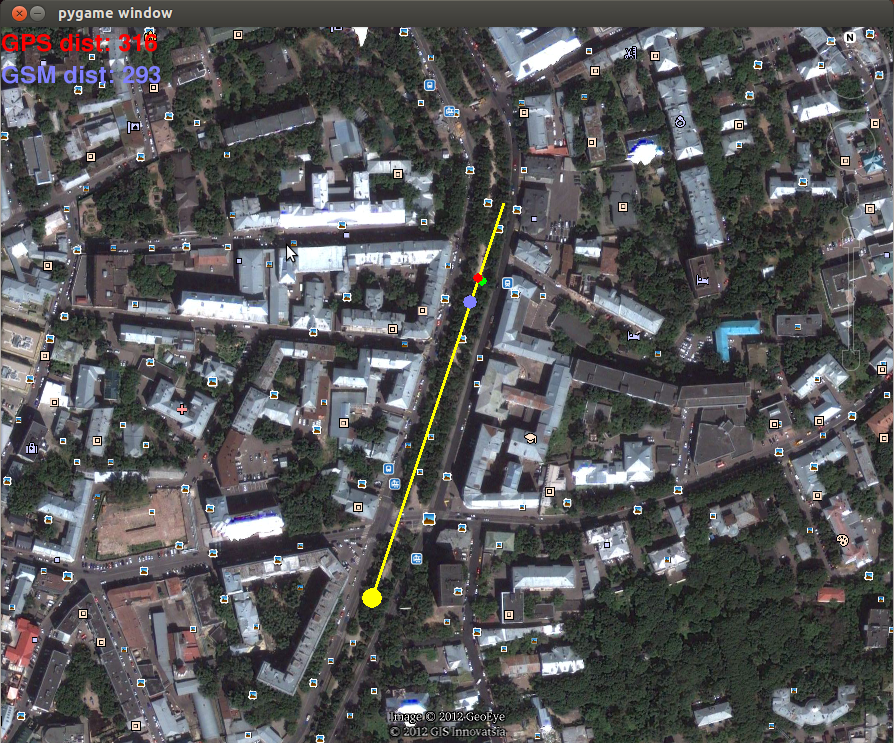
\includegraphics[width=\textwidth]{gfront-gsm-mode.png}
				\caption{Позиционирование}
			}
			\label{subfig:gfront-gsm-mode}
		\end{subfigure}
	}
	\caption{Снимки работы графического клиента в двух возможных режимах. Изображение местности взято из приложения Google Earth\cite{googleearth} на условиях Fair use\cite{enwikifairuse}.}
	\label{fig:gfront}
\end{figure}

Данное приложение отображает на экране вид сверху на местность, где осуществлялось тестирование приложения (снимок взят из приложения Google Earth\cite{googleearth} на условиях Fair use\cite{enwikifairuse}), поверх которого рисует жёлтым цветом линию маршрута, обозначив его начало кругом того же цвета (см. рис. \ref{fig:gfront}).

Приложение, будучи запущенным, открывает соединение с сервером по протоколу TCP и начинает ждать передачи данных. При приходе сообщения в формате JSON, клиент определяет режим работы сервера по содержимому принятого сообщения (см. подпункты \ref{subsubsec:server-collect-frontend} и \ref{subsubsec:server-perform-main}), после чего сам переключается в соответствующий режим (менять режим возможно с каждым новым пакетом, если это потребуется).

\subsection{Режим сбора данных}
В режиме сбора данных (рис. \ref{fig:gfront}\subref{subfig:gfront-gps-mode}) клиент отображает на карте зелёной точкой истинное положение мобильного устройства по данным GPS, а голубой --- её проекцию на маршрут. На экране отображается параметр Dist, означающий расстояние в метрах от начала маршрута до проекции положения мобильного устройства на него, и Err --- расстояние от истинного положения до его проекции на маршрут в метрах.

\subsection{Режим позиционирования}
В режиме позиционирования (рис. \ref{fig:gfront}\subref{subfig:gfront-gsm-mode}) клиент отображает на карте:
\begin{itemize}
	\item
		{\bf{}Зелёная точка} --- истинное положение устройства по данным GPS;
	\item
		{\bf{}Красная точка} --- проекция истинного положения на маршрут;
	\item
		{\bf{}Голубая точка} --- результат позиционирования по данным GSM.
\end{itemize}

Параметры GPS dist и GSM dist означают расстояние от начала маршрута до положения устройства по данным GPS и GSM соответственно.
